%
% Presentación para el video "La cuota de mi hipoteca está mal calculada"
%
% ©Esta obra, cuyo autor es Antonio Araúzo Azofra, está bajo una licencia 
% de Reconocimiento-CompartirIgual 4.0 Internacional de Creative Commons
%
\documentclass{beamer}
\usepackage{beamerthemeshadow}
%\usetheme{default}%Ilmenau}
%\usecolortheme{whale}%whale
\usepackage[utf8]{inputenc}
\usepackage[spanish]{babel}
\usepackage{eurosym}
\DeclareUnicodeCharacter{20AC}{\euro}
\newcommand{\putat}[3]{\begin{picture}(0,0)(0,0)\put(#1,#2){#3}\end{picture}}
\usepackage{fancybox}

\definecolor{links}{HTML}{2A1B81}
\hypersetup{colorlinks,linkcolor=,urlcolor=links}

% Decimal columns
\usepackage{siunitx}
\sisetup{%
  obeyall,
}


% To get text at absolute position with a callout: http://tex.stackexchange.com/questions/18821/pop-up-effect-in-beamer
\usepackage[absolute,overlay]{textpos}
\usepackage{tikz}
\usetikzlibrary{shadows}

%**
% \PutAt<overlay spec>[<box width>]{(<x>, <y>)}{<content>}
%
% real absolute positioning of <content> on a slide, if content is a figure,
% minipage or whatever kind of LR-box, the <box width> argument may be omitted
%
% implementation notes: 
%   - based on   \usepackage[absolute,overlay]{textpos}
%   - NOT combinable with any beamer feature that is based on pgfpages
%     (such as dual-screen support, built-in 2up handouts, etc.), as textpos 
%     and pgfpates interfere at the shippout-level.
%
  \newcommand<>{\PutAt}[3][0pt]{%
    {\only#4{\begin{textblock*}{#1}#2%
      #3%
    \end{textblock*}}}%
  }
%**
% \ShowPutAtGrid
%
% draws a helpful grid on the current slide to figure <x> and <y> parameters for \PutAt
% 
  \newcommand{\ShowPutAtGrid}{
    \begin{textblock*}{128mm}(0cm,0cm)
    \tikz[color=red!20!white]\draw[very thin, step=5mm] (0mm,0mm) grid (130mm,100mm);
    \end{textblock*}
    \begin{textblock*}{128mm}(0cm,0cm)
    \begin{tikzpicture}[color=red]
      \draw[step=1cm] (0,0mm) grid (130mm,100mm);   
      \foreach \n in {0,...,12}
        \draw[xshift=.5mm,yshift=-1.5mm, inner sep=0pt, anchor=west] (\n,10) node {\scriptsize{\textbf{\n}}};
      \foreach \n in {1,...,9}
        \draw[xshift=.5mm,yshift=-1.5mm, inner sep=0pt, anchor=west] (0,10-\n) node {\scriptsize{\textbf{\n}}};
    \end{tikzpicture}
    \end{textblock*}
  }
%**
% \NormalBox<overlay spec>[tikz picture/node options]{<content>}
%
% draws content boxed in a nice box
% 
\newcommand<>{\NormalBox}[2][]{%
  \only#3{\tikz[#1, every node/.style={shape=rectangle,draw,fill=white, drop shadow, #1}]\node []{#2};}
}
%**
% \OrangeBox<overlay spec>[tikz picture/node options]{<content>}
%
% draws content boxed in an orange call-out box
% 
\newcommand<>{\OrangeBox}[2][]{%
  \onslide#3{\NormalBox[fill=yellow,draw=black!30,rounded corners=4pt,#1]{#2}}%
} 





\begin{document}
%gets rid of navigation symbols
\setbeamertemplate{navigation symbols}{}

\title{La cuota de mi hipoteca está mal calculada}  
\author{ \raisebox{-0.8ex}{
\includegraphics[height=3ex]{by-sa.pdf}} \hspace{2cm} Antonio Araúzo Azofra}
\date{\today} 

{
\usebackgroundtemplate{\bigskip \bigskip \hbox to \paperwidth{\hfil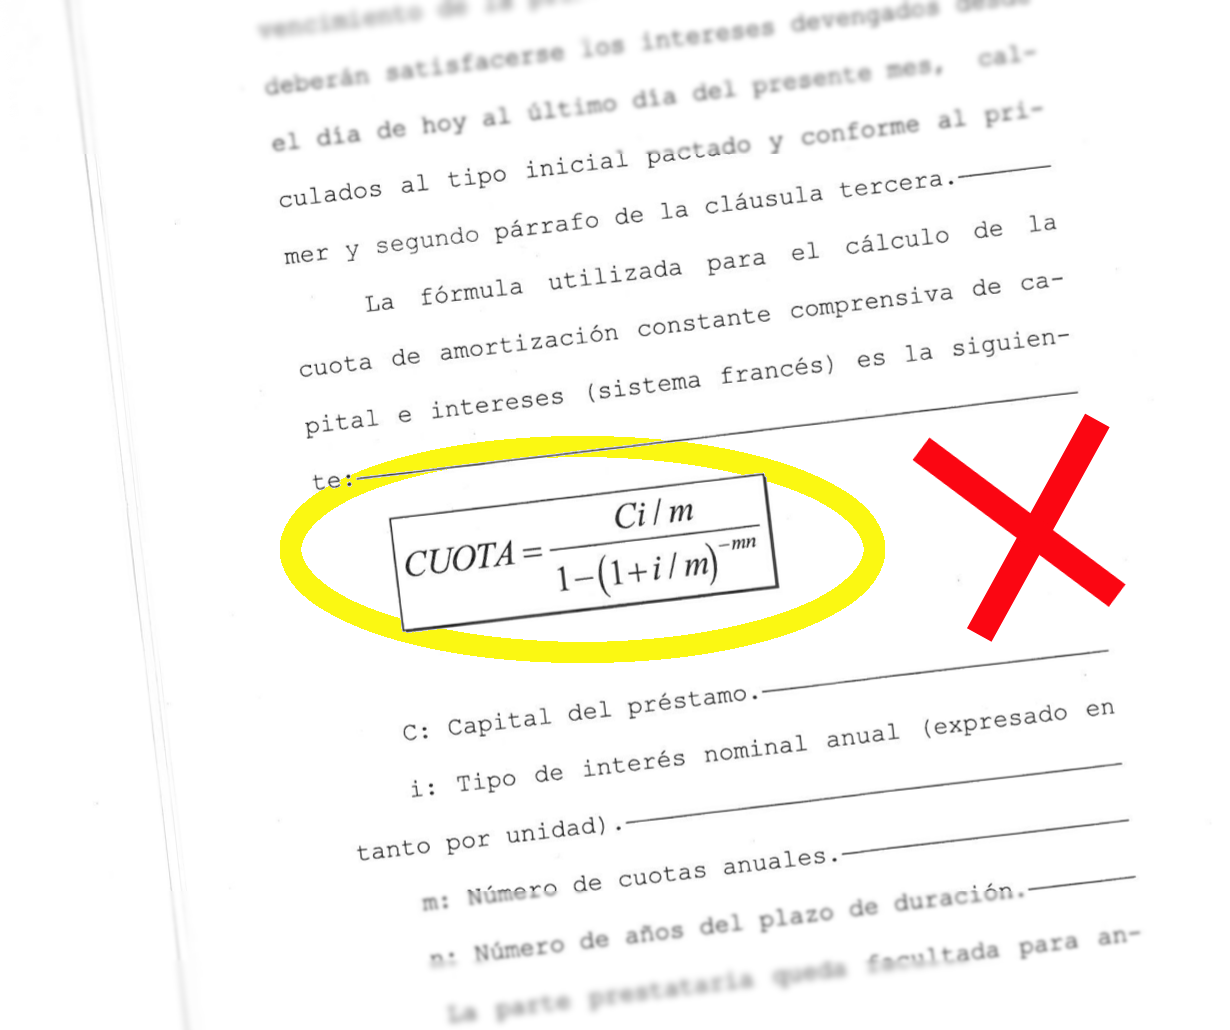
\includegraphics[height=\paperheight]{EscaneadoHojaFormula.png}\hfil}}
\frame{\frametitle{\bf La cuota de mi hipoteca está mal calculada}}
}



%gets rid of bottom navigation bars
\setbeamertemplate{footline}{}

\frame{\frametitle{Tu cuota probablemente también\\(hipoteca o préstamo, que ya tengas o vayas a tener...)}
\begin{columns}
  \pause
  \begin{column}{0.48\textwidth}
      \setbeamercolor{block title}{use=structure,fg=white,bg=red!75!black}
      %\setbeamercolor{block body}{use=structure,fg=black,bg=red!20!white}
      \begin{block}{\center \bf Aproximada}
%      \resizebox{!}{23pt}{
          \setlength\abovedisplayskip{0pt}
          \vspace{1mm}
          \LARGE
          \begin{equation*}
          m = C \frac{ \frac{i}{12} } {1 - \frac{1}{(1+\frac{i}{12})^{12n}}}
          \end{equation*}
          \vspace{1mm}
          %suponen $i_m = \frac{i}{12}$
%      }
      \end{block}
  \end{column}
  \pause
  \begin{column}{0.48\textwidth}
      \setbeamercolor{block title}{use=structure,fg=white,bg=green!75!black}
      %\setbeamercolor{block body}{use=structure,fg=black,bg=red!20!white}
      \begin{block}{\center \bf Exacta}
%      \resizebox{!}{23pt}{
          \setlength\abovedisplayskip{0pt}
          \vspace{2mm}
          \LARGE
          \begin{equation*}
          m = C \frac{\sqrt[12]{(1+i)}-1}{1-\frac{1}{(1+i)^{n}}}
          \end{equation*}
          \vspace{2mm}
          %donde $i_m = (1+i)^{\frac{1}{12}} - 1$
%      }
      \end{block}
  \end{column}
\end{columns}
}



\frame{\frametitle{Interés simple}
\begin{center}
$C_\text{ Final} = C_\text{ Inicial} \cdot (1+i \cdot t)$
\end{center}
\smallskip
\pause
\begin{center} 
  \includegraphics[width=\textwidth]{IntSimple1.pdf} 
\end{center}
}

\frame{\frametitle{Interés simple}
\begin{center}
$C_\text{ Final} = C_\text{ Inicial} \cdot (1+i \cdot t)$
\end{center}
\smallskip
\begin{center} 
  \includegraphics[width=\textwidth]{IntSimple2.pdf} 
\end{center}
}

\frame{\frametitle{Interés simple}
\begin{center}
$C_\text{ Final} = C_\text{ Inicial} \cdot (1+i \cdot t)$
\end{center}
\smallskip
\begin{center} 
  \includegraphics[width=\textwidth]{IntSimple3.pdf} 
\end{center}
}

\frame{\frametitle{Interés simple}
\begin{center}
$C_\text{ Final} = C_\text{ Inicial} \cdot (1+i \cdot t)$
\end{center}
\smallskip
\begin{center} 
  \includegraphics[width=\textwidth]{IntSimple4.pdf} 
\end{center}
}

\frame{\frametitle{Interés simple}
\begin{center}
$C_\text{ Final} = C_\text{ Inicial} \cdot (1+i \cdot t)$
\end{center}
\smallskip
\begin{center} 
  \includegraphics[width=\textwidth]{IntSimple5.pdf} 
\end{center}
}

\frame{\frametitle{Interés simple}
\begin{center}
$C_\text{ Final} = C_\text{ Inicial} \cdot (1+i \cdot t)$
\end{center}
\smallskip
\begin{center} 
  \includegraphics[width=\textwidth]{IntSimple6.pdf} 
\end{center}
}

\frame{\frametitle{Interés simple}
\begin{center}
$C_\text{ Final} = C_\text{ Inicial} \cdot (1+i \cdot t)$
\end{center}
\smallskip
\begin{center} 
  \includegraphics[width=\textwidth]{IntSimple7.pdf} 
\end{center}
}

\frame{\frametitle{Interés simple}
\begin{center}
$C_\text{ Final} = C_\text{ Inicial} \cdot (1+i \cdot t)$
\end{center}
\smallskip
\begin{center} 
  \includegraphics[width=\textwidth]{IntSimple8.pdf} 
\end{center}
}

\frame{\frametitle{Interés simple}
\begin{center}
$C_\text{ Final} = C_\text{ Inicial} \cdot (1+i \cdot t)$
\end{center}
\smallskip
\begin{center} 
  \includegraphics[width=\textwidth]{IntSimple9.pdf} 
\end{center}
}

\frame{\frametitle{Interés simple}
\begin{center}
$C_\text{ Final} = C_\text{ Inicial} \cdot (1+i \cdot t)$
\end{center}
\smallskip
\begin{center} 
  \includegraphics[width=\textwidth]{IntSimple.pdf} 
\end{center}
\PutAt<2->{(0.5cm,3cm)}{
  \rotatebox{35}{
    \OrangeBox[font=\LARGE]{\bf ¡No sirve para comparar!}
  }
}
% Intento de poner un circulo amarillo para destacar
%\PutAt<+>{(10cm,7.5cm)}{
%\setlength{\unitlength}{1cm}
%\begin{picture}(2,0.5)
%\linethickness{1mm}
%\color{yellow}
%\qbezier(1, 0)(3, 0.25)(1, 0.5)
%\qbezier(1, 0)(-1, 0.25)(1, 0.5)
%\end{picture}
%}
%\ShowPutAtGrid
}



\frame{\frametitle{Interés compuesto}
\begin{center}
$C_\text{ Final} = C_\text{ Inicial} \cdot (1+i)^t$
\end{center}
\pause
\smallskip
\begin{center} 
  \includegraphics[width=\textwidth]{IntCompuesto1.pdf} 
\end{center}
}

\frame{\frametitle{Interés compuesto}
\begin{center}
$C_\text{ Final} = C_\text{ Inicial} \cdot (1+i)^t$
\end{center}
\smallskip
\begin{center} 
  \includegraphics[width=\textwidth]{IntCompuesto.pdf} 
\end{center}
}

\frame{\frametitle{Interés compuesto}
\begin{center}
$C_\text{ Final} = C_\text{ Inicial} \cdot (1+i)^t$
\end{center}
\smallskip
\begin{center} 
  \includegraphics[width=\textwidth]{IntCompuesto2.pdf} 
\end{center}
\pause
\PutAt<+->{(0.5cm,1cm)}{
  \rotatebox{20}{
    \NormalBox[font=\LARGE]{\bf VAN}
  }
}
\PutAt<+->{(2.3cm,2cm)}{
  \rotatebox{10}{
    \NormalBox[font=\LARGE]{\bf TIR}
  }
}
\PutAt<+->{(4cm,1.5cm)}{
  \rotatebox{15}{
    \NormalBox[font=\LARGE]{\bf Rentabilidad bonos}
  }
}
\PutAt<+->{(7.5cm,2cm)}{
  \rotatebox{10}{
    \NormalBox[font=\LARGE]{\bf Prima de riesgo}
  }
}
}



\frame{\frametitle{¿Qué pasa con los préstamos?}}
%26
\frame{\frametitle{¿Qué pasa con los préstamos?}
\bigskip
{\renewcommand{\arraystretch}{1.018}
\begin{tabular}{rSSSS}
\hline
{\it Pago} & {\it Deuda} & {\it Interés} & {\it Amortización}  & {\it Cuota}\hspace{0.5cm} \\ \hline
0 & 1000.00 &       & & \\ \hline
1 &         & 50.00 & & \\ \hline
2 & & & & \\ \hline
3 & & & & \\ \hline
4 & & & & \\ \hline
5 & & & & \\ \hline
6 & & & & \\ \hline
7 & & & & \\ \hline
8 & & & & \\ \hline
9 & & & & \\ \hline
10& & & & \\ \hline
\end{tabular}
}
\begin{textblock*}{7cm}(1cm,2cm)
\begin{tikzpicture}
\draw[opacity=0] (0cm,0cm) -- (7cm,-6cm); 
\draw[->,blue,line width=1pt] (2.75cm,-0.75cm) -- node[above,pos=0.9] {\small 5\%} (4cm,-1cm);
\end{tikzpicture}
\end{textblock*}
}
%27
\frame{\frametitle{¿Qué pasa con los préstamos?}
\bigskip
{\renewcommand{\arraystretch}{1.018}
\begin{tabular}{rSSSS}
\hline
{\it Pago} & {\it Deuda} & {\it Interés} & {\it Amortización}  & {\it Cuota}\hspace{0.5cm} \\ \hline
0 & 1000.00 &       & & \\ \hline
1 &         & 50.00 &  79.50 & 129.50 \\ \hline
2 & & & & \\ \hline
3 & & & & \\ \hline
4 & & & & \\ \hline
5 & & & & \\ \hline
6 & & & & \\ \hline
7 & & & & \\ \hline
8 & & & & \\ \hline
9 & & & & \\ \hline
10& & & & \\ \hline
\end{tabular}
}
\begin{textblock*}{7cm}(1cm,2cm)
\begin{tikzpicture}
\draw[opacity=0] (0cm,0cm) -- (7cm,-6cm); 
\draw[->,blue,line width=1pt] (2.75cm,-0.75cm) -- node[above,pos=0.9] {\small 5\%} (4cm,-1cm);
\draw[blue, inner sep=0pt, anchor=center] (5cm, -1.28cm) node {\small{\textbf{+}}};
\draw[blue, inner sep=0pt, anchor=center] (7cm, -1.28cm) node {\small{\textbf{=}}};
\end{tikzpicture}
\end{textblock*}
}
% 28
\frame{\frametitle{¿Qué pasa con los préstamos?}
\bigskip
{\renewcommand{\arraystretch}{1.018}
\begin{tabular}{rSSSS}
\hline
{\it Pago} & {\it Deuda} & {\it Interés} & {\it Amortización}  & {\it Cuota}\hspace{0.5cm} \\ \hline
0 & 1000.00 &       & & \\ \hline
1 &  920.50 & 50.00 &  79.50 & 129.50 \\ \hline
2 & & & & \\ \hline
3 & & & & \\ \hline
4 & & & & \\ \hline
5 & & & & \\ \hline
6 & & & & \\ \hline
7 & & & & \\ \hline
8 & & & & \\ \hline
9 & & & & \\ \hline
10& & & & \\ \hline
\end{tabular}
}
\begin{textblock*}{7cm}(1cm,2cm)
\begin{tikzpicture}
\draw[opacity=0] (0cm,0cm) -- (7cm,-6cm); 
\draw[->,blue,line width=1pt] (2.75cm,-0.75cm) -- node[above,pos=0.9] {\small 5\%} (4cm,-1cm);
\draw[blue, inner sep=0pt, anchor=center] (5cm, -1.28cm) node {\small{\textbf{+}}};
\draw[blue, inner sep=0pt, anchor=center] (7cm, -1.28cm) node {\small{\textbf{=}}};
\draw[->,blue,line width=1pt] (5.6cm,-1.4cm) -- (5.5cm,-1.5cm) -- (3cm,-1.5cm) -- (2.75cm,-1.25cm);
\end{tikzpicture}
\end{textblock*}
}
% 29
\frame{\frametitle{¿Qué pasa con los préstamos?}
\bigskip
{\renewcommand{\arraystretch}{1.018}
\begin{tabular}{rSSSS}
\hline
{\it Pago} & {\it Deuda} & {\it Interés} & {\it Amortización}  & {\it Cuota}\hspace{0.5cm} \\ \hline
0 & 1000.00 &       & & \\ \hline
1 &  920.50 & 50.00 &  79.50 & 129.50 \\ \hline
2 &         & 46.02 &  83.48 & 129.50 \\ \hline
3 & & & & \\ \hline
4 & & & & \\ \hline
5 & & & & \\ \hline
6 & & & & \\ \hline
7 & & & & \\ \hline
8 & & & & \\ \hline
9 & & & & \\ \hline
10& & & & \\ \hline
\end{tabular}
}
\begin{textblock*}{7cm}(1cm,2cm)
\begin{tikzpicture}
\draw[opacity=0] (0cm,0cm) -- (7cm,-6cm); 
\draw[->,blue,line width=1pt] (2.75cm,-0.75cm) -- node[above,pos=0.9] {\small 5\%} (4cm,-1cm);
\draw[blue, inner sep=0pt, anchor=center] (5cm, -1.28cm) node {\small{\textbf{+}}};
\draw[blue, inner sep=0pt, anchor=center] (7cm, -1.28cm) node {\small{\textbf{=}}};
\draw[->,blue,line width=1pt] (5.6cm,-1.4cm) -- (5.5cm,-1.5cm) -- (3cm,-1.5cm) -- (2.75cm,-1.25cm);
\draw[blue, inner sep=0pt, anchor=center] (5cm, -1.78cm) node {\small{\textbf{+}}};
\draw[blue, inner sep=0pt, anchor=center] (7cm, -1.78cm) node {\small{\textbf{=}}};
\draw[->,blue,line width=1pt] (2.25cm,-1.5cm) -- node[below,pos=0.15] {\small 5\%} (3.5cm,-1.75cm);
\end{tikzpicture}
\end{textblock*}
}
%30
\frame{\frametitle{¿Qué pasa con los préstamos?}
\bigskip
{\renewcommand{\arraystretch}{1.018}
\begin{tabular}{rSSSS}
\hline
{\it Pago} & {\it Deuda} & {\it Interés} & {\it Amortización}  & {\it Cuota}\hspace{0.5cm} \\ \hline
0 & 1000.00 & & & \\ \hline
1 & 920.50 & 50.00 &  79.50 & 129.50\\ \hline
2 & 837.02 & 46.02 &  83.48 & 129.50\\ \hline
3 & 749.36 & 41.85 &  87.65 & 129.50\\ \hline
4 & 657.33 & 37.47 &  92.04 & 129.50\\ \hline
5 & 560.69 & 32.87 &  96.64 & 129.50\\ \hline
6 & 459.22 & 28.03 & 101.47 & 129.50\\ \hline
7 & 352.67 & 22.96 & 106.54 & 129.50\\ \hline
8 & 240.80 & 17.63 & 111.87 & 129.50\\ \hline
9 & 123.34 & 12.04 & 117.46 & 129.50\\ \hline
10&   0.00 &  6.17 & 123.34 & 129.50\\ \hline
\end{tabular}
}
\begin{textblock*}{7cm}(1cm,2cm)
\begin{tikzpicture}
\draw[opacity=0] (0cm,0cm) -- (7cm,-6cm); 
\draw[->,blue,line width=1pt] (2.75cm,-0.75cm) -- node[above,pos=0.9] {\small 5\%} (4cm,-1cm);
\draw[blue, inner sep=0pt, anchor=center] (5cm, -1.28cm) node {\small{\textbf{+}}};
\draw[blue, inner sep=0pt, anchor=center] (7cm, -1.28cm) node {\small{\textbf{=}}};
\draw[->,blue,line width=1pt] (5.6cm,-1.4cm) -- (5.5cm,-1.5cm) -- (3cm,-1.5cm) -- (2.75cm,-1.25cm);
\draw[blue, inner sep=0pt, anchor=center] (5cm, -1.78cm) node {\small{\textbf{+}}};
\draw[blue, inner sep=0pt, anchor=center] (7cm, -1.78cm) node {\small{\textbf{=}}};
\end{tikzpicture}
\end{textblock*}
}



\frame{\frametitle{Cálculo de la cuota}
\begin{columns}<1->
  \begin{column}{0.28\textwidth}
  \end{column}
  \begin{column}{0.35\textwidth}
      \setbeamercolor{block title}{use=structure,fg=white,bg=blue!75!black}
      \begin{block}{\center \bf Cuota fija\\(método frances)}
        \setlength\abovedisplayskip{0pt}
        \Large
        \begin{equation*}
        a = C \frac{i}{1-\frac{1}{(1+i)^n}}
        \end{equation*}
%        { \footnotesize
%        \begin{itemize}
%        \item $a$, cuota fija (anualidad)
%        \item $C$, capital
%        \item $i$, tipo de interés (anual)
%        \item $n$, número de pagos (años)
%        \end{itemize}
%        }
      \end{block}
  \end{column}
  \begin{column}{0.28\textwidth}
  \end{column}
\end{columns}
\bigskip

\only<2->{
\PutAt[3cm]{(2cm,2.8cm)}{\large $i_m = \frac{i_a}{12}$} 
\begin{textblock*}{1.5cm}(2.8cm,3.3cm)
\begin{tikzpicture}
\draw[->,red!75!black,line width=1mm] (1.5cm, 0cm) .. controls (0.5cm,-0.5cm) .. (0cm, -1.5cm);
\end{tikzpicture}
\end{textblock*}
}

\only<4->{
\PutAt[4cm]{(9cm,2.8cm)}{\large $i_m = \sqrt[12]{(1+i)}-1$} 
\begin{textblock*}{1.5cm}(8.45cm,3.3cm)
\begin{tikzpicture}
\draw[->,green!75!black,line width=1mm] (0cm, 0cm) .. controls (1cm,-0.5cm) .. (1.5cm, -1.5cm);
\end{tikzpicture}
\end{textblock*}
}

\begin{columns}
  \begin{column}{0.48\textwidth}<3->
      \setbeamercolor{block title}{use=structure,fg=white,bg=red!75!black}
      %\setbeamercolor{block body}{use=structure,fg=black,bg=red!20!white}
      \begin{block}{\center \bf Aproximada}
%      \resizebox{!}{23pt}{
          \setlength\abovedisplayskip{0pt}
          \vspace{1mm}
          \LARGE
          \begin{equation*}
          m = C \frac{ \frac{i}{12} } {1 - \frac{1}{(1+\frac{i}{12})^{12n}}}
          \end{equation*}
          \vspace{1mm}
          %suponen $i_m = \frac{i}{12}$
%      }
      \end{block}
  \end{column}
  \pause
  \begin{column}{0.48\textwidth}<5->
      \setbeamercolor{block title}{use=structure,fg=white,bg=green!75!black}
      %\setbeamercolor{block body}{use=structure,fg=black,bg=red!20!white}
      \begin{block}{\center \bf Exacta}
%      \resizebox{!}{23pt}{
          \setlength\abovedisplayskip{0pt}
          \vspace{2mm}
          \LARGE
          \begin{equation*}
          m = C \frac{\sqrt[12]{(1+i)}-1}{1-\frac{1}{(1+i)^{n}}}
          \end{equation*}
          \vspace{2mm}
          %donde $i_m = (1+i)^{\frac{1}{12}} - 1$
%      }
      \end{block}
  \end{column}
\end{columns}
}



\frame{\frametitle{¿Qué diferencia hay entre ambas?}
%\ShowPutAtGrid
\PutAt<2->[\paperwidth]{(0cm,0cm)}{
\begin{tikzpicture}[remember picture,overlay]
   \node[at=(current page.center)]{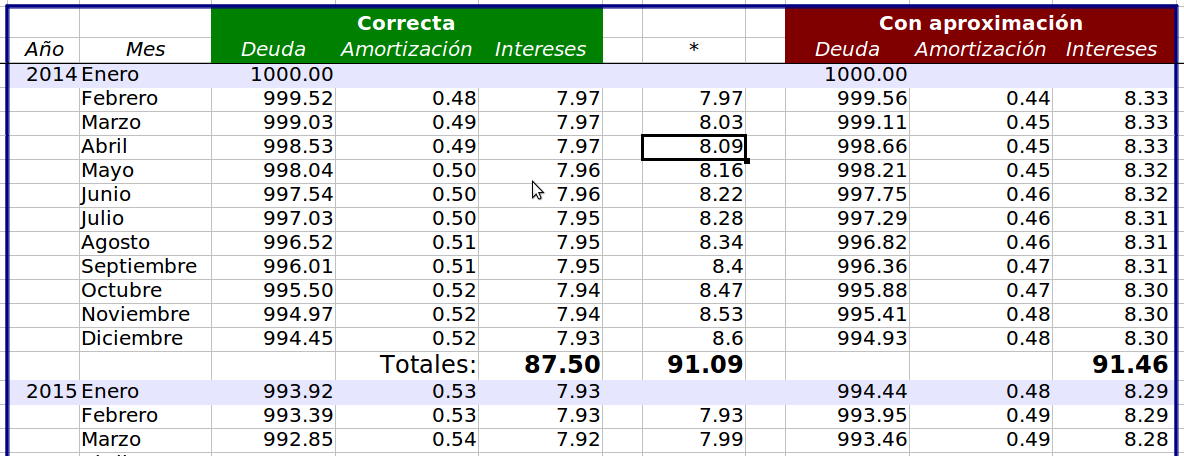
\includegraphics[width=12cm]{ScreenshotInteresesSobreIntereses.png}};
   \node[at=(current page.center),yshift=-2.5cm]{$\vdots$};
\end{tikzpicture}
}
\PutAt<3->[\paperwidth]{(0cm,0cm)}{
\begin{tikzpicture}[remember picture,overlay]
\draw[->,blue,line width=1mm] (7.65cm,-2cm) -- (7.65,-3.3cm);
\end{tikzpicture}
}
}



\frame{\frametitle{¿Por qué usan la aproximación?}
%\ShowPutAtGrid
\begin{columns}
  \begin{column}{0.85\textwidth}
    \begin{enumerate}
    \item<2-> ¿Más fácil?
        \begin{itemize}
        \item En el pasado, vale. Hoy en día, hasta el teléfono que llevamos encima puede hacer miles de estos cálculos en un segundo.
%        \item Aplicaciones para móvil en nuestra web: \href{http://interes.ax5.org/}{interes.ax5.org}
        \end{itemize}
    \item<4-> ¿Tradición?
        \begin{itemize}
        \item Las tradiciones están bien para las fiestas pero ¿usar una aproximación tipo ``cuenta la vieja'' por tradición?
        \end{itemize}
    \item<6-> ¿Ignorancia?
        \begin{itemize}
        \item No, en los bancos hay gente muy preparada haciendo cálculos mucho más complejos que estos.
        \end{itemize}
    \item<8-> ¿Más beneficios para el banco?
        \begin{itemize}
        \item Esta aproximación siempre resulta en mayores ingresos para el banco.
        \end{itemize}
    \end{enumerate}
  \end{column}
  \begin{column}{0.1\textwidth}
        \bigskip
        
        \visible<3->{\begin{tikzpicture}
        \draw[red,line width=2mm] (0cm,0cm) -- (1cm,1cm);
        \draw[red,line width=2mm] (0cm,1cm) -- (1cm,0cm);
        \end{tikzpicture}}

        \bigskip
        \visible<5->{\begin{tikzpicture}
        \draw[red,line width=2mm] (0cm,0cm) -- (1cm,1cm);
        \draw[red,line width=2mm] (0cm,1cm) -- (1cm,0cm);
        \end{tikzpicture}}

        \bigskip
        \visible<7->{\begin{tikzpicture}
        \draw[red,line width=2mm] (0cm,0cm) -- (1cm,1cm);
        \draw[red,line width=2mm] (0cm,1cm) -- (1cm,0cm);
        \end{tikzpicture}}

        \bigskip
        \visible<9->{\centering \fontsize{2cm}{1em}\selectfont \color{blue} \bf ?}
  \end{column}
\end{columns}
}



\frame{\frametitle{¿Por qué es importante que se use la exacta?}
\begin{itemize}
    \item Permitiria hipotecas TAE / Nobasta con que se publique el TAE
    \pause
    \item Crece cuanto más crece
    \pause
    \item Claro y sencillo, el interés anual equivalente permite comparar con depósitos y cualquier otro producto financiero
\end{itemize}
}


\frame{\frametitle{-Eliminar-}
\begin{itemize}
    \item donde $a$ es la cuota fija o anualidad, $C$ es el capital, $i$ el tipo de interés anual y $n$ el número de años
    \item ¿Cómo debe calcularse una mensualidad?
    \item $i = (1+i_t)^{\frac{1}{n}} - 1$    
\end{itemize}
}








%\frame{\frametitle{References / Referencias} 
%\small
%ISO/IEC Guide 23:1982 \url{http://www.iso.org/iso/iso_iec_guide_23_1982.pdf}
%\bigskip

%\bigskip
%\scriptsize
%Pictures used from:
%\tiny
%\begin{itemize}
%\item 
%\end{itemize}
%}

\end{document}
